% !TEX root = ../apprentissage.tex
\section{Conclusion}

\begin{frame}{Conclusion}
%  \begin{itemize}
%    \item de tout temps l'évolution technique à eu des détracteur
%    \item l'éducation connait un décalage avec les besoins sociétal (nivean TIC)
%    \item ce décalage empêche l'arrivé des jeunes sur le marché de l'emploi
%    \item ce décalage favorise l'échec scolaire
%    \item ainsi que des drames liée à la mauvaise utilisation des NTIC
%    \item depuis le début de 20ème siècle de nombreuse initiative sont née   
%  \end{itemize}
   \begin{center}
     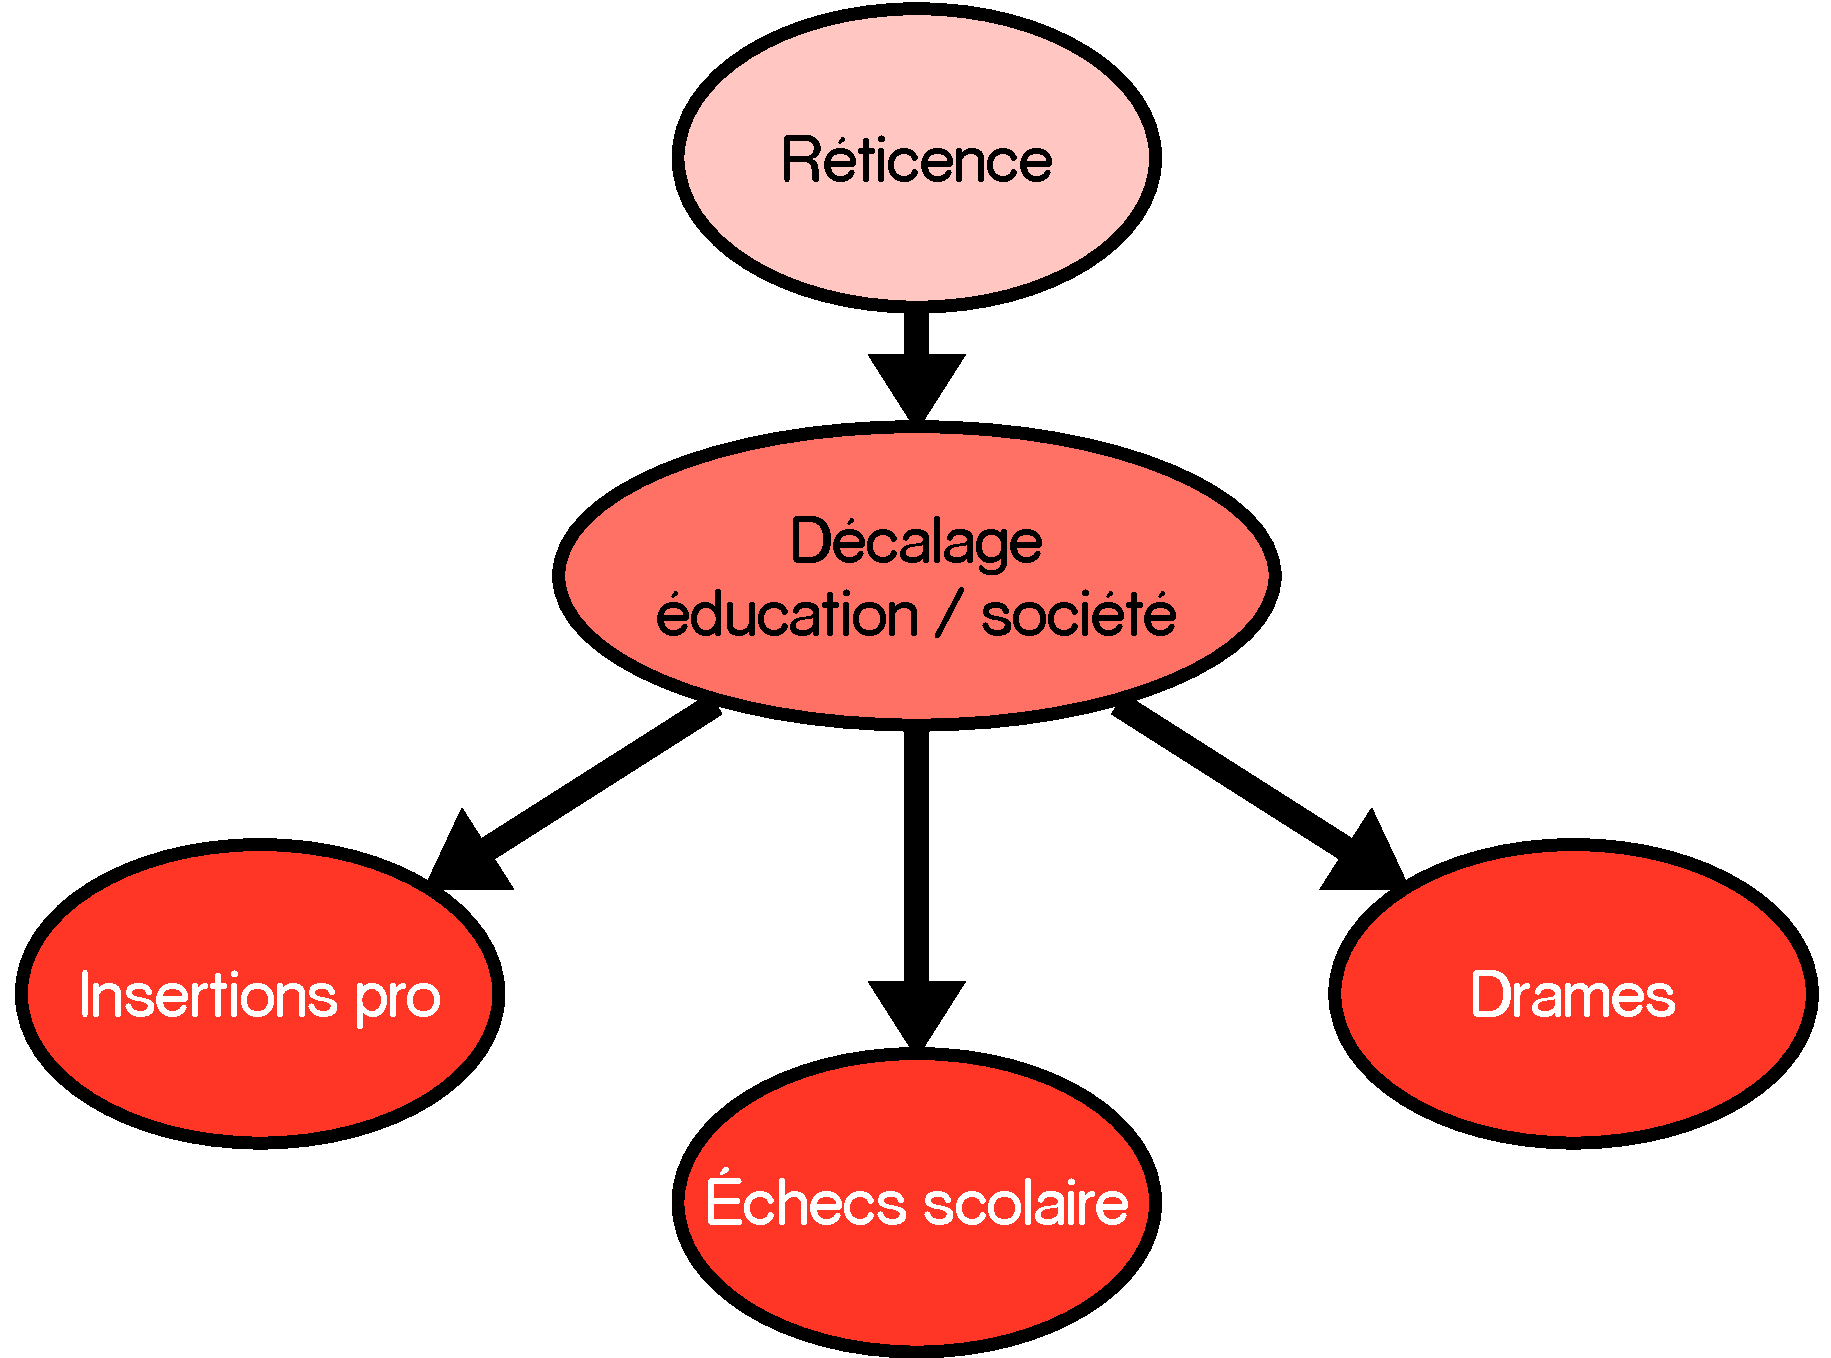
\includegraphics[width=.7\textwidth]{../resources/illustrations/ccl}
   \end{center}
\end{frame}

\begin{frame}{Concrètement}
\begin{itemize}
  \item Projets vs. Problèmes
  \item Multiniveaux
  \item Multidisciplinaires
  \item D'abord confronter l'élève à la problématique avant de lui enseigner les concepts abstraits
\end{itemize}
\end{frame}

\begin{frame}{Ouverture}
  \vfill
    \begin{block}{Neurosciences}
    \begin{itemize}
    \item Faire un résumé en fin de cours
    \item Création de carte mentale
    \end{itemize}
  \end{block}
  \vfill
  \begin{center}
    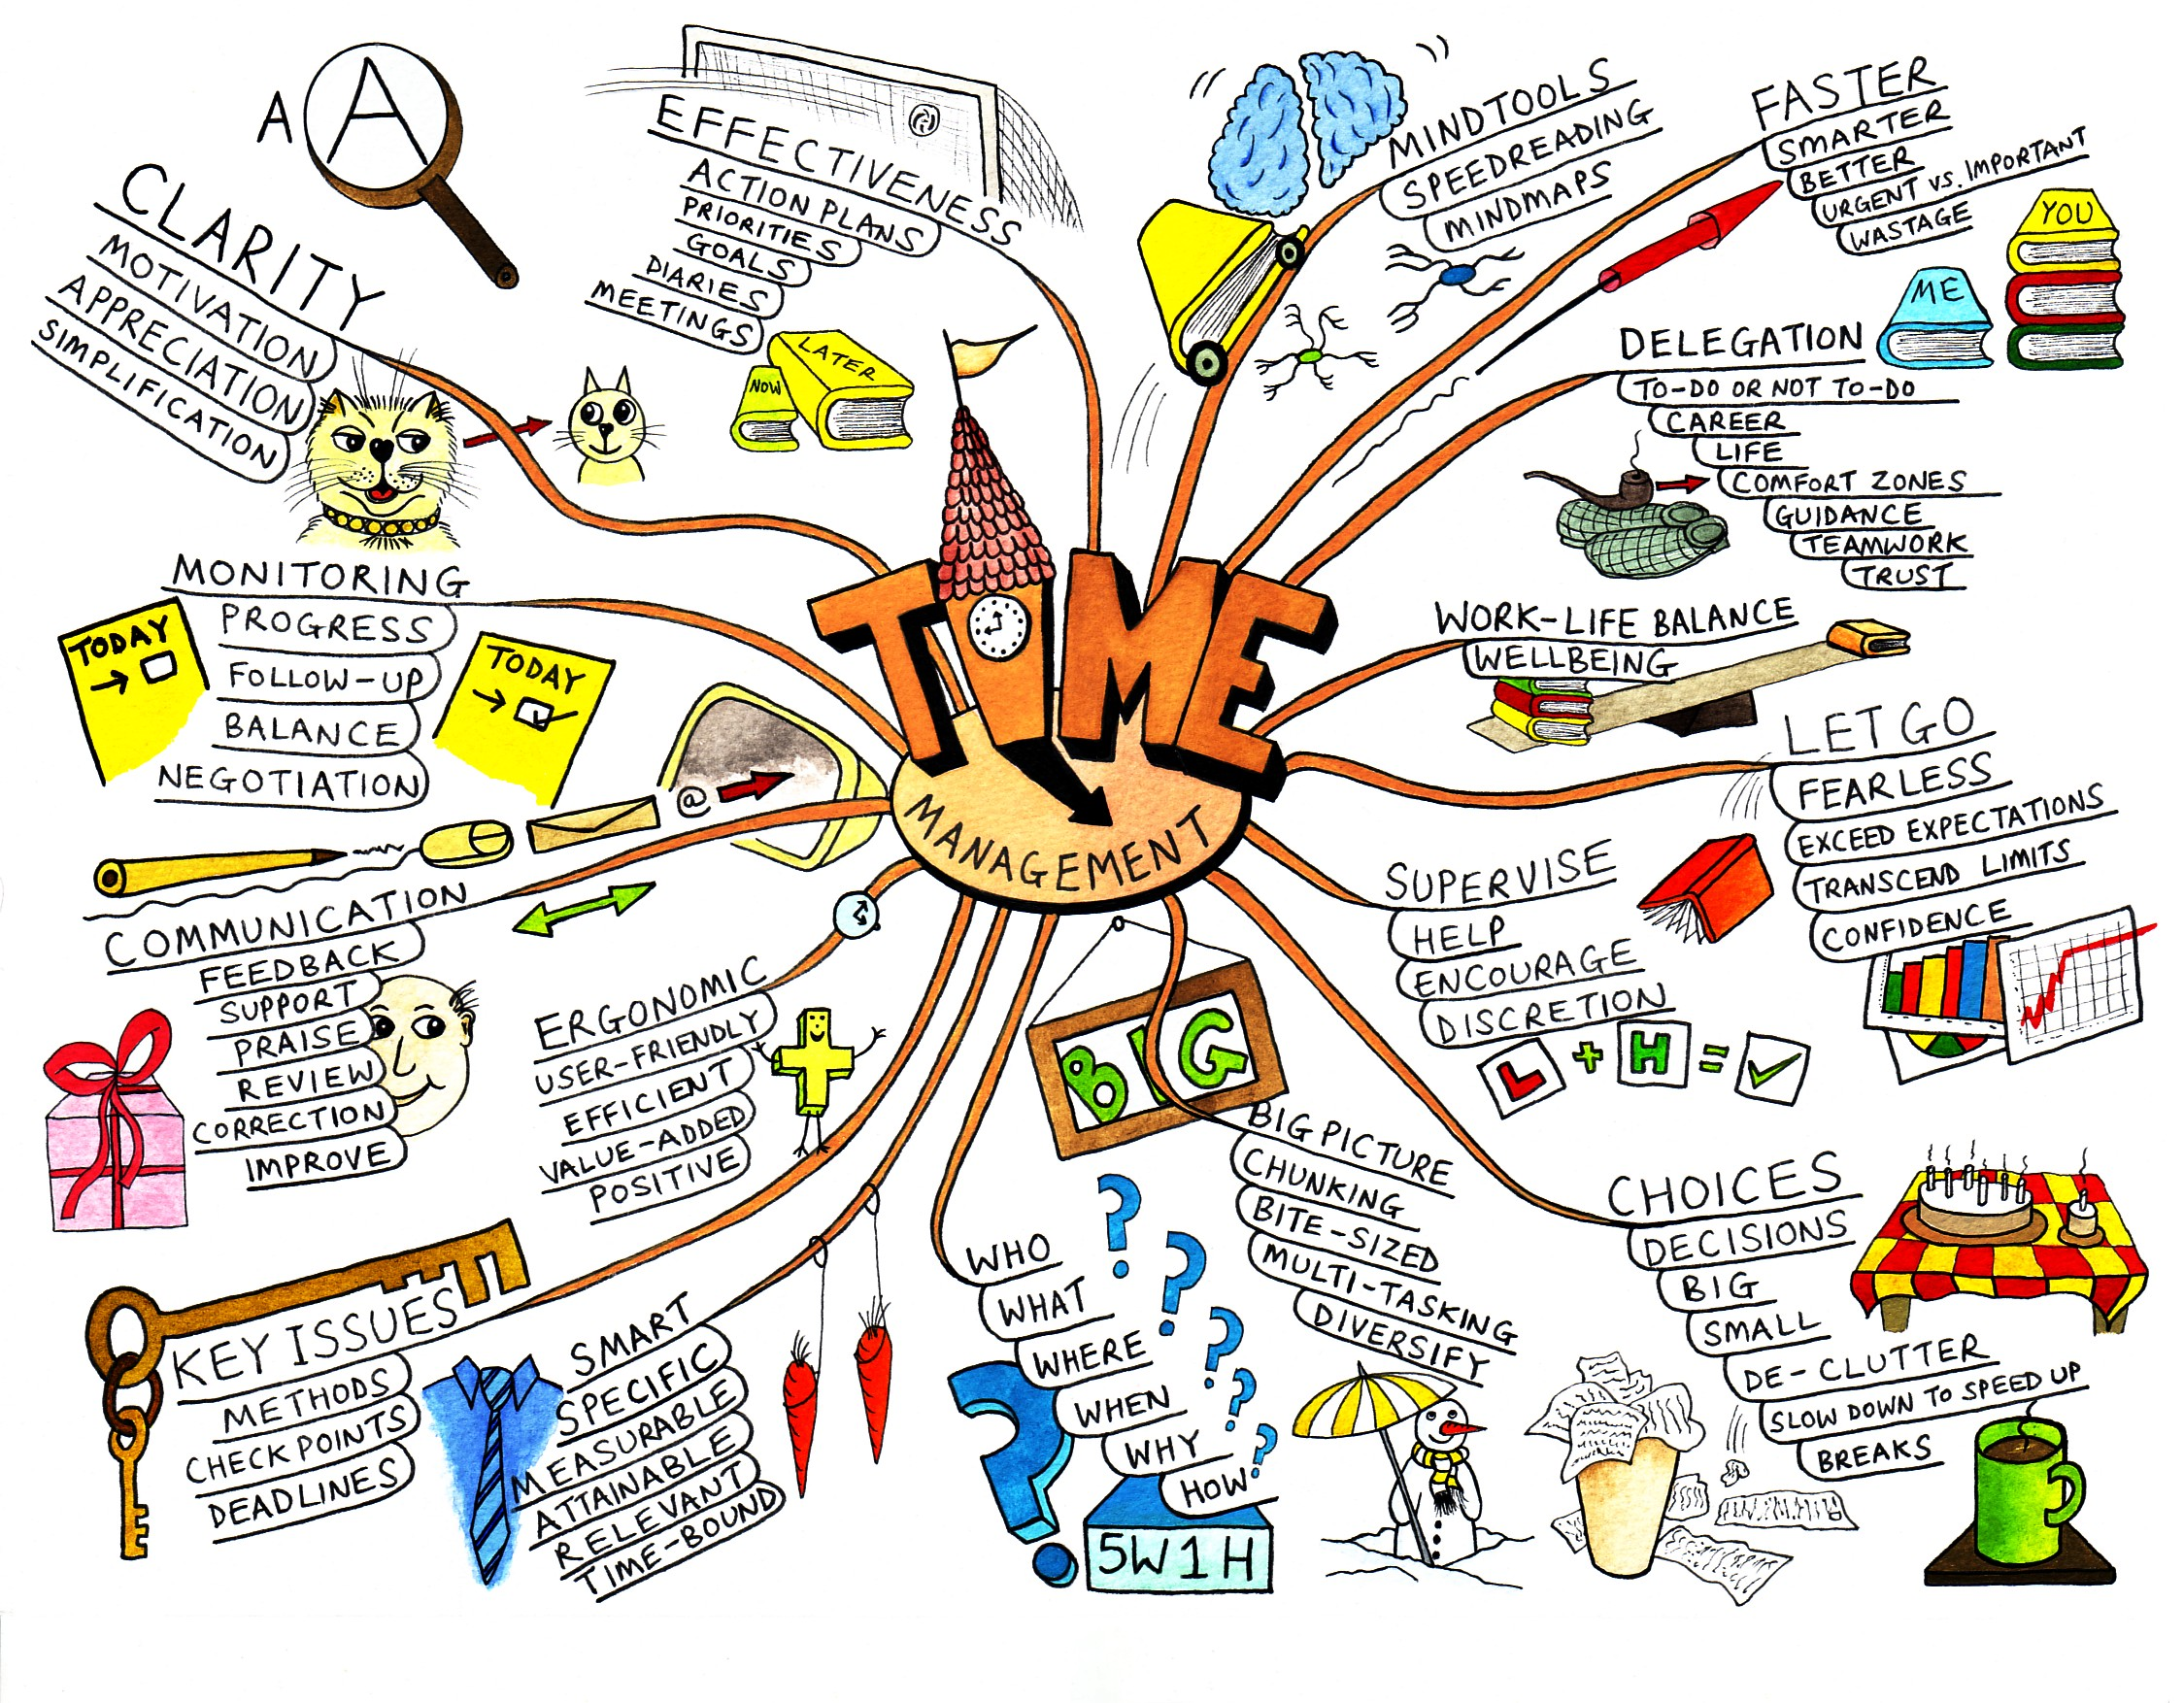
\includegraphics[width=.6\textwidth]{../resources/illustrations/mindmap.jpg}
  \end{center}
    \vfill
  \footlineextra{\cite{neurosup}}
\end{frame}

\begin{frame}
\Huge
\begin{center}
	Merci pour votre attention !
	
	Avez-vous des questions ?
	\includegraphicsabsolute{../resources/illustrations/seymour_skinner_2}{4cm}{.3cm}{6cm}
\end{center}
\end{frame}

